\section{Methods}

\paragraph{Model}
Convolutional networks' architectures for image recognition have evolved quite drastically in recent years,
with numerous options available "out of the box".
E.g.\ Efficient Net (EffNet) delivers impressive accuracy, while being able to scale better than a lot of
previous architectures~\cite{DBLP:journals/corr/abs-1905-11946}.
For this paper, the evaluation was done using it, namely EfficientNetB0~\cite{KerasEffNet}

\paragraph{Rotation pretext task}
A common choice of pretext task could be to produce 4 copies of
a single image by rotating it by {0°, 90°, 180°, 270°} and let a single network predict the rotation which was applied.
Alexander Kolesnikov and Xiaohua Zhai and Lucas Beyer: "Intuitively, a good model should learn to
recognize canonical orientations of objects in natural images" ~\cite{kolesnikov2019revisiting}.
For this papers evaluation, each image from the original dataset was rotated 0°, 90°, 180°,
270° and assigned a new pseudo label from [0, 1, 2, 3] accordingly.
The examples of such images are shown in~\ref{fig:rot-fig}.
All 4 batches of rotated images, as well as pseudo labels were concatenated in new dataset, and shuffled.
Then EffNet was then trained to identify rotation applied, afterwards the convolutional layers were frozen,
and the output layer size was adjusted for the downstream task \footnote{For details about pretext tasks implementations please refer to
impl/util/pretext.py in accompanying GitHub repository~\cite{github} \label{fn-pre}}.

\begin{figure}[h]
    \begin{subfigure}{0.33\textwidth}
        \caption{Label = 0}
        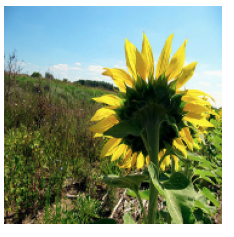
\includegraphics[width=5cm]{images/rot_0}
    \end{subfigure}
    \begin{subfigure}{0.2\textwidth}
        \caption{Label = 1}
        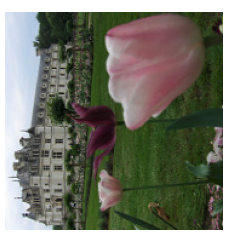
\includegraphics[width=5cm]{images/rot_1}
    \end{subfigure}
    \begin{subfigure}{0.33\textwidth}
        \caption{Label = 2}
        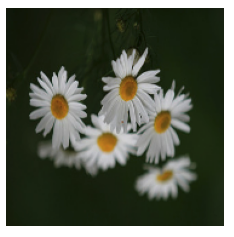
\includegraphics[width=5cm]{images/rot_2}
    \end{subfigure}
    \caption{An example how images used for rotation pretext task could look like}
    \label{fig:rot-fig}
\end{figure}


\paragraph{Jigsaw pretext task}
The task is
to recover relative spatial position of 4 sampled image patches
after a random permutation of these patches was performed
~\cite{kolesnikov2019revisiting}.
All of these patches are concatenated in 'puzzle' image,
which is later sent through the same network, which needs to predict a permutation applied.\
A similar approach as described by Mehdi Noroozi and Paolo Favaro~\cite{DBLP:journals/corr/NorooziF16} was adopted.
Random 4 out of 24 possible permutations were chosen for each batch
(number of possible permutations can be obtained from Newtonian binomial $P=\frac{r!}{(r-n)!}$).
For each permutation, each image was cut in 4 equal parts,
afterwards these tiles were permuted as per chosen permutation, and concatenated in 1 (puzzle) image.
An example can be seen in~\ref{fig:jig-fig}.
Similarly, to rotation pseudo labels in [0\ldots23] had been assigned,
NN was trained to identify permutation applied.
Then the weights of convolutional layers were frozen and reused for the downstream task ^{\ref{fn-pre}}.

\\
\begin{figure}[h]
    \begin{subfigure}{0.33\textwidth}
        \caption{Original image}
        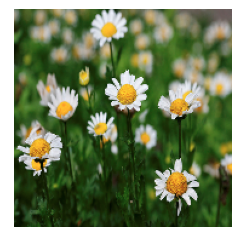
\includegraphics[width=5cm]{images/dandelion}
    \end{subfigure}
    \begin{subfigure}{0.2\textwidth}
        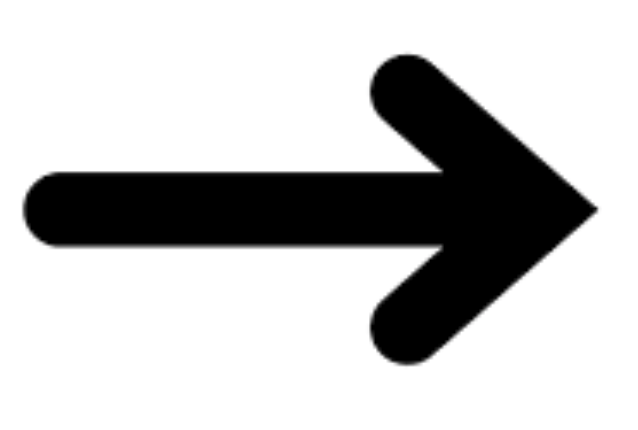
\includegraphics[width=3cm]{images/arrow}
    \end{subfigure}
    \begin{subfigure}{0.33\textwidth}
        \caption{Generated puzzle, label=1}
        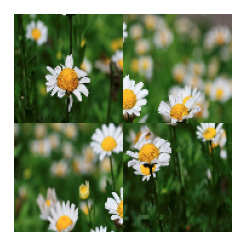
\includegraphics[width=5cm]{images/puzzle}
    \end{subfigure}
    \caption{An example how puzzle for jigsaw pretext task could look like}
    \label{fig:jig-fig}
\end{figure}


\paragraph{Transfer Learning}For this paper, EffNet was pre-trained on "imagenette"~\cite{ImageNette} dataset for image classification.
Imagenette is a subset of 10 easily classified classes from the Imagenet dataset.
Afterwards, the NN was fine-tuned for an actual classification task of interest on~\cite{tfflowers}.

\paragraph{Adversarial Images with FGSM}
The implementation of FGSM for this paper was based on~\cite{FGSM}.
In order to generate an adversarial pattern for each image, as per previously described formula~\ref{eq:adv}
gradient of loss function is evaluated with sign for each image.
Then as per previously described approach,
an adversarial pattern was added pixel wise to the original image with $\epsilon = 0.01$.
The resulting adversarial image was then clipped by value, so each channels' value stays in interval [0\ldots255],
as required for RGB color encoding
\footnote{For details about adversarial attack implementation please refer to
impl/util/adversarial.py in accompanying GitHub repository~\cite{github} \label{fn-adv}}.


\newpage
\paragraph{Evaluation approach}
In order to evaluate, how including pretext task in the training process influences NNs vulnerability against adversarial attacks,
I have measured miss-classification rate while keeping the intensity of adversarial pattern fixed at $\epsilon = 0.01$.
\\
Following metrics of interest were recorded:

\begin{equation}
    Accuracy_i = \frac{\# \; images \; correctly \; classified_i}{\# \; test \; images_i} \cdot 100 \%
\end{equation} \\
where Accuracy\_i is the accuracy in each evaluation round \\
\# stands for "number".

\begin{equation}
    Miss \; rate_i = \frac{\# images \; miss \; classified_i}{\# \; images \; correctly \; classified_i} \cdot 100 \%
\end{equation}
where Miss rate\_i is the miss rate in each evaluation round.


The dataset "tf\_flowers"~\cite{tfflowers} was chosen for experiment, 5\% of dataset were reserved for evaluation.
\\
During each evaluation round NN network was pre-trained either with transfer learning, or rotation, or jigsaw.
The number of training epochs was varied in [15, 30, 45, 60] for pretext training, while the number of epochs for downstream
training was fixed at 30.
\\
The reserved for evaluation images were given to NN. The number of correct classifications was recorded.
Then, for each previously correctly classified image FGSM~\ref{eq:adv} with $\epsilon = 0.01$ was applied.
The number of miss-classifications was recorded afterwards \footnote{For details about evaluation implementations please refer to
impl/util/evaluation.py in accompanying GitHub repository~\cite{github} \label{fn-eval}}.

